\documentclass[10pt,norsk,a4paper]{article}
\usepackage[utf8]{inputenc}
\usepackage[T1]{fontenc}
\usepackage[norsk]{babel}
\usepackage[cm]{fullpage}
\usepackage{color}
\usepackage{parskip,textcomp,amssymb,graphicx}
\usepackage{pdfpages}

\title{Generalforsamling\\
	Vår 2017\\
	Cybernetisk Selskab\\[.3cm]
	
\includegraphics[width=0.8\textwidth]{cyblogoa3.pdf}\\[-.5cm]}
\date{10. november 2016}

\begin{document}
\maketitle{}
\tableofcontents{}

%\newpage
~\\

\section{Valg av møteleder}

\section{Valg av referent}

\section{Valg av protokollunderskrivere}

\section{Valg av tellekorps}

\section{Godkjenning av innkalling}

\section{Godkjenning av dagsorden}

\newpage


\section{Semesterberetninger}
\subsection{Semesterberetning ved Leder}

Blir lagt inn som vedlegg under Generalforsamlingen.

%\newpage


\subsection{Semesterberetning ved Kjellermogul}

Blir lagt inn som vedlegg under Generalforsamlingen.

\newpage

\section{Regnskap}
Kasserer orientere om regnskap\\

%\newpage


\section{Revidert budsjett vår 2017}
Kasserer orientere om budsjett\\


\newpage

\section{Kontingentfastsettelse}
Hovedstyret foreslår å holde medlemskontigenten på 30 kroner.\\

\section{Valg}

\begin{minipage}[t]{9cm}
\subsection{Hovedstyret}
Man velges inn i hovedstyret for ett år av gangen.
\subsubsection{Leder}

\subsubsection{Nestleder}

\subsubsection{Rekrutteringsansvarlig}

\end{minipage}
\begin{minipage}[t]{9cm}
\subsection{Kjellerstyret}
Alle verv som er til valg i kjellerstyret, gjelder for ett semester av gangen.

\subsubsection{Barsjef}

\subsubsection{Innkjøpsansvarlig}

\subsubsection{Kafésjef}

\subsubsection{Teknisk ansvarlig}

\subsubsection{DJ-sjef}

\subsubsection{Utlånsansvarlig}

\end{minipage}

%\newpage
\newpage

\section{Vedtektsendringer}
\subsection($\mathsection5$h)
Hovedstyret ønsker å legge til:\\
Hovedstyret må bestå av minimum 2/3 ifi-studenter.

\section{Æresmedlemskap}

\section{Utdeling av pins}
Arkivar deler ut pins\\

\section*{Vedlegg: Vedtekter}

\newpage

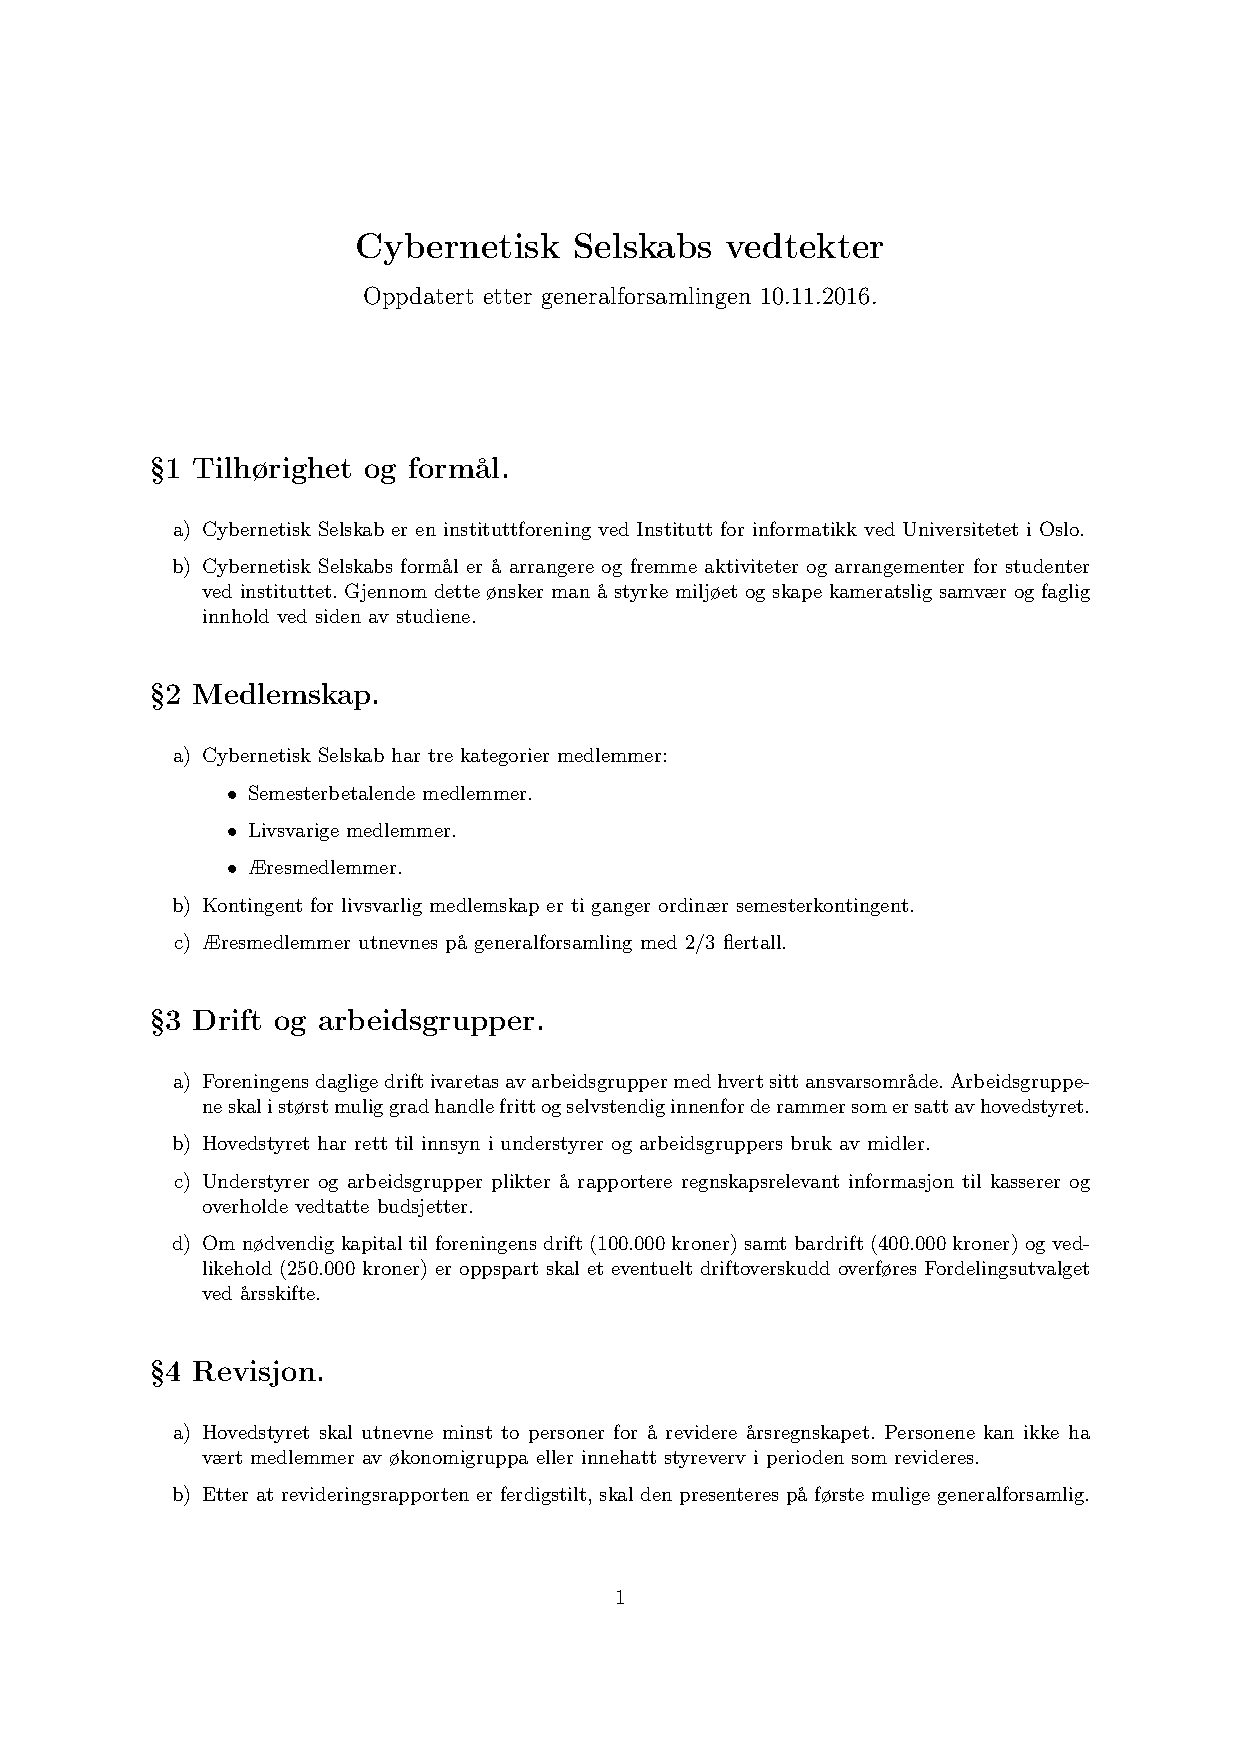
\includepdf[pages=-]{cyb_vedtekter.pdf}
\end{document}
